\documentclass[
	aspectratio=169, % default is 43
	8pt, % font size, default is 11pt
	handout, % handout mode without animations, comment out to add animations
]{beamer}

\usepackage{../template/beamerthemeuulm} % use the inofficial uulm beamer theme
\setfaculty{infIngPsy} % set the color scheme for your faculty here [med/infIngPsy/math/nat]

% requires symbolic links
% git clone git@github.com:SoftVarE-Group/SlideTemplate.git C:\Users\...\SlideTemplate
% mklink /J template C:\Users\...\SlideTemplate
% git clone git@spgit.informatik.uni-ulm.de:thuem/slides.git C:\Users\...\ThomasSlides
% mklink /J thomasslides C:\Users\...\ThomasSlides
\graphicspath{{../template/pics/logos}{../template/pics/nature}{../template/pics/uulm}{../thomasslides/}{../pics/people/}{../pics/xkcd/}}

%\usepackage[ngerman]{babel} % use this line for slides in German
%\recordingtrue % special recording mode for use with a greenscreen, gives you space to show yourself in a layer in front of the slides, has no effect in the handout mode

\title{Software Product Lines} % short title is used for the slide footer but optional

% LINKED LITERATURE

\newcommand{\ludewiglichter}{\href{https://learning.oreilly.com/library/view/-/9781457184932/?ar}{Ludewig and Lichter}}
\newcommand{\seeconomics}{\href{https://rds-ulm.ibs-bw.de/link?kid=027381854}{SE Economics}}
\newcommand{\sommervillelink}[1]{\href{https://ulm.ibs-bw.de/aDISWeb/app?service=direct/0/Home/$DirectLink\&sp=SOPAC00\&sp=SAKSWB-IdNr1615420983}{#1}}
\newcommand{\sommerville}{\sommervillelink{Sommerville}}
\newcommand{\thehumbleprogrammer}{\href{https://dl.acm.org/doi/10.1145/1283920.1283927}{The Humble Programmer}}
\newcommand{\thepragmaticprogrammer}{\href{https://learning.oreilly.com/library/view/the-pragmatic-programmer/9780135956977/}{The Pragmatic Programmer}}

% TYPICAL COMMANDS FOR LECTURES

\renewcommand{\emph}[1]{{\color{blue}\textbf{#1}}}

\newcommand{\deutsch}[1]{{\color{blue}(#1)}}
\newcommand{\deutschertitel}[1]{{\tiny\deutsch{#1}}}

\newcommand{\mycite}[1]{``#1''}
\newcommand{\mytitlesource}[1]{{\tiny\normalfont\mbox{[#1]}}}
\newcommand{\mysource}[1]{\ifthenelse{\equal{#1}{}}{}{\phantom{.}~\hfill~\mytitlesource{#1}}}

\newcommand{\todo}[1]{{\color{red}\textbf{[#1]}}}
\newcommand{\fodo}[1]{\todo{\footnote{\todo{#1}}}}
\newcommand{\todots}{\todo{\ldots}}

% IMPORTED PACKAGES

%\usepackage{adjustbox} % used for partofpage
%\usepackage{tcolorbox} % used for mydefinition, mynote, myexample
\usepackage{multicol} % used temporarily for the lecture overview
\usepackage{mathtools} % required for absolute value in modeling lecture

% COMMANDS TO LAYOUT AND ANNIMATE SLIDES

\newcommand{\lessonslearned}[3]{
	\subsection{Summary}
	\begin{frame}{\insertsection -- \insertsubsection}
		\leftorright{
			\mydefinition{Lessons Learned}{
				\begin{itemize}
					#1
				\end{itemize}
			}
			\mynote{Further Reading}{
				\small % references take space, can be a little smaller
				\begin{itemize}
					#2
				\end{itemize}
			}
		}{
			\myexample{Practice}{
				#3
			}
		}
	\end{frame}
}

% TODO temporary hack to layout the slide overview in two colums
\renewcommand{\lectureoverview}{
%	\section*{Overview}
%	\subsection*{Overview}
	\begin{frame}{\insertsubtitle}
		\begin{multicols}{2}
			\tableofcontents
		\end{multicols}
	\end{frame}
}

\renewcommandx{\maketitle}[2][1=apr21-o25a,2=150]{
    {
	\usebackgroundtemplate{} % TODO temporary hack to enable missing pictures at title slide
	%\ifx {#1} \empty \else {\usebackgroundtemplate{\includegraphics[trim=0 0 0 #2,clip,width=\paperwidth]{#1}}} \fi     
	%\usebackgroundtemplate{\includegraphics[trim=0 0 0 #2,clip,width=\paperwidth]{#1}}
    \begin{frame}[plain]
        \vskip0pt plus 1filll
        \begin{beamercolorbox}[wd=\paperwidth,ht=4.5ex,dp=2ex,right]{titlebox}
            \LARGE\textbf{\inserttitle}\hspace*{20pt}
        \end{beamercolorbox}%
        \nointerlineskip%
        \begin{beamercolorbox}[wd=\paperwidth,ht=2.25ex,dp=1ex,right]{subtitlebox}
            \small 
            \ifx \insertsubtitle \empty \else \insertsubtitle\ $\vert$ \fi
            \insertauthor\
            \ifx \insertdate \empty \else $\vert$ \insertdate \fi
            \hspace*{20pt}
        \end{beamercolorbox}%
        \nointerlineskip%
        \begin{beamercolorbox}[wd=\paperwidth,ht=4.5ex,dp=2ex,left]{logobox}
            \centering
            \vspace{-1ex}
            \hspace{10pt}
            \includegraphics[height=4.5ex]{sp} % SPECIFY INSTITUTE LOGO HERE
            \hfill
            \includegraphics[height=4.5ex]{uulm}
            \hspace{10pt}
        \end{beamercolorbox}%
    \end{frame}
    }  
}

%
%\newcommand{\onlyleft}[1]{
%	\halfpage{#1}
%}
%
%\newcommand{\onlyright}[1]{
%	~\hfill
%	\halfpage{#1}
%}
%
%\newcommand{\leftorright}[2]{
%	\uncover<1>{\halfpage{#1}}
%	\hfill
%	\uncover<3->{\halfpage{#2}}
%}
%
%\newcommand{\rightorleft}[2]{
%	\uncover<3->{\halfpage{#1}}
%	\hfill
%	\uncover<1>{\halfpage{#2}}
%}
%
%\newcommand{\leftthenright}[2]{
%	\halfpage{#1}
%	\hfill\pause
%	\halfpage{#2}
%}
%
%\newcommand{\leftandright}[2]{
%	\halfpage{#1}
%	\hfill
%	\halfpage{#2}
%}
%
%\newcommand{\leftmiddleandright}[3]{
%	\thirdpage{#1}
%	\hfill
%	\thirdpage{#2}
%	\hfill
%	\thirdpage{#3}
%}
%
%\newcommand{\leftmiddleorright}[3]{
%	\uncover<1>{\thirdpage{#1}}
%	\hfill
%	\uncover<3>{\thirdpage{#2}}
%	\hfill
%	\uncover<5->{\thirdpage{#3}}
%}
%
%\newcommand{\halfpage}[1]{\partofpage{48}{#1}}
%
%\newcommand{\thirdpage}[1]{\partofpage{31}{#1}}
%
%\newcommand{\partofpage}[2]{
%	\adjustbox{valign=t}{\begin{minipage}{0.#1\textwidth}
%			\begin{flushleft}
%				#2
%			\end{flushleft}
%	\end{minipage}}
%}
%
%\newcommand{\mydefinition}[2]{
%	\begin{tcolorbox}[title=#1,colback=orange!10,colframe=orange!30,coltitle=black,fonttitle=\bfseries,left=1mm,right=1mm,top=1mm,bottom=1mm]
%		\begin{flushleft}
%			#2
%		\end{flushleft}
%	\end{tcolorbox}
%}
%
%\newcommand{\mydefinitiontight}[2]{
%	\begin{tcolorbox}[title=#1,colback=white,colframe=orange!30,coltitle=black,fonttitle=\bfseries,left=0mm,right=0mm,top=0mm,bottom=0mm]
%		\begin{flushleft}
%			#2
%		\end{flushleft}
%	\end{tcolorbox}
%}
%
%\newcommand{\mynote}[2]{
%	\begin{tcolorbox}[title=#1,colback=red!10,colframe=red!30,coltitle=black,fonttitle=\bfseries,left=1mm,right=1mm,top=1mm,bottom=1mm]
%		\begin{flushleft}
%			#2
%		\end{flushleft}
%	\end{tcolorbox}
%}
%
%\newcommand{\myexample}[2]{
%	\begin{tcolorbox}[title=#1,colback=blue!10,colframe=blue!30,coltitle=black,fonttitle=\bfseries,left=1mm,right=1mm,top=1mm,bottom=1mm]
%		\begin{flushleft}
%			#2
%		\end{flushleft}
%	\end{tcolorbox}
%}
%
%\newcommand{\myexampletight}[2]{
%	\begin{tcolorbox}[title=#1,colback=white,colframe=blue!30,coltitle=black,fonttitle=\bfseries,left=0mm,right=0mm,top=0mm,bottom=0mm]
%		\begin{flushleft}
%			#2
%		\end{flushleft}
%	\end{tcolorbox}
%}
% TYPICAL COMMANDS FOR LECTURES

\renewcommand{\emph}[1]{{\color{blue}\textbf{#1}}}

\newcommand{\deutsch}[1]{{\color{blue}(#1)}}
\newcommand{\deutschertitel}[1]{{\tiny\deutsch{#1}}}

\newcommand{\mycite}[1]{``#1''}
\newcommand{\mycitebegin}{``}
\newcommand{\myciteend}{''}
\newcommand{\mytitlesource}[1]{{\tiny\normalfont\mbox{[#1]}}}
\newcommand{\mysource}[1]{\ifthenelse{\equal{#1}{}}{}{\phantom{.}~\hfill~\mytitlesource{#1}}}
\newcommand{\mypage}[1]{, p.~#1}
\newcommand{\mypages}[1]{, pp.~#1}

\newcommand{\todo}[1]{{\color{red}\textbf{[#1]}}}
\newcommand{\fodo}[1]{\todo{\footnote{\todo{#1}}}}
\newcommand{\todots}{\todo{\ldots}}

\newcommand{\textheightwithtitle}{.825\textheight}
\newcommand{\textheightwithouttitle}{.975\textheight}

\newcommand{\lessonslearned}[3]{
	\subsection{Summary}
	\begin{frame}{\insertsection{} -- \insertsubsection}
		\leftandright{
			\mydefinition{Lessons Learned}{
				\begin{itemize}
					#1
				\end{itemize}
			}
			\uncover<2->{\mynote{Further Reading}{
				\small % references take space, can be a little smaller
				\begin{itemize}
					#2
				\end{itemize}
			}}
		}{
			\uncover<3->{\myexample{Practice}{
				\begin{itemize}
					#3
				\end{itemize}
			}}
		}
	\end{frame}
}

% COMMANDS FOR PROPOSITIONAL FORMULAS AND MATHEMATICAL NOTATIONS

\newcommand{\sem}[1]{\ensuremath{\llbracket #1 \rrbracket}} % semantics brackets
\newcommand{\pand}{\wedge} % conjunction
\newcommand{\por}{\vee} % disjunction
\newcommand{\pnot}{\neg} % negation
\newcommand{\pequals}{\leftrightarrow} % biconditional
\newcommand{\npequals}{\nleftrightarrow} % exclusive disjunction
\newcommand{\mequals}{\Leftrightarrow} % equivalence (meta-level)
\newcommand{\pimplies}{\rightarrow} % conditional
\newcommand{\mimplies}{\Rightarrow} % implication (meta-level)
\newcommand{\defeq}{\vcentcolon=} % defining equals
\newcommand{\power}[1]{\mathcal{P}(#1)} % power set
\newcommand{\refslide}[1]{\hyperlink{#1}{(see Slide \autoref{#1})}} % link to slide
\newcommand{\fs}[1]{\ensuremath{{\color{green}#1}}} % selected feature
\newcommand{\fd}[1]{\ensuremath{{\color{red}#1}}} % deselected feature
\newcommand{\cfg}[3][0]{\ensuremath({{\only<#1>{\color{green}}\{#2\}}, {\only<#1>{\color{red}}\{#3\}})}} % configuration

\usepackage{mathtools} % required for absolute value in modeling lecture
\DeclarePairedDelimiter\abs{\lvert}{\rvert} % absolute value

% COMMANDS TO INCLUDE XKCDs

\newcommand{\xkcd}[2]{
	\href{https://xkcd.com/#1/}{\includegraphics[#2]{#1}}
}
\newcommand{\xkcdframe}[1]{
	\begin{frame}
		\centering%
		\xkcd{#1}{height=80mm}
	\end{frame}
}
\newcommand{\widexkcdframe}[1]{
	\begin{frame}
		\xkcd{#1}{width=\linewidth}
	\end{frame}
}

% COMMANDS TO SIMPLIFY USAGE OF THE PROJECT CARTOON

\newcommand{\projectcartoonwidth}{.19} % default value for 5 tiles
\newcommand{\projectcartoon}[2]{\projectcartoonimage{sepia/cell_#1}{#2}}
\newcommand{\hprojectcartoon}[2]{\projectcartoonimage{alpha/cell_#1}{#2}}
\newcommand{\projectcartoonimage}[2]{
	\begin{minipage}[t]{\projectcartoonwidth\linewidth}
		\centering
		\href{http://web.archive.org/web/20191029221320/http://www.projectcartoon.com/}{\includegraphics[width=\linewidth]{#1}}\\#2
	\end{minipage}\hfill
}
\newcommand{\waterfallcartoon}{
	\hprojectcartoon{02}{Analysis}%
	\hprojectcartoon{03}{Design}%
	\hprojectcartoon{04}{Implementation}%
	\hprojectcartoon{05}{Testing}%
	\hprojectcartoon{10}{Maintenance}%
}
%\uncover<1->{\hprojectcartoon{01}{how the customer explained it}} % requirements
%\uncover<1->{\hprojectcartoon{02}{how the project leader understood it}} % modeling
%\uncover<1->{\hprojectcartoon{03}{how the analyst designed it}} % architecture and design
%\uncover<1->{\hprojectcartoon{04}{how the programmer implemented it}} % implementation
%\uncover<1->{\hprojectcartoon{05}{what the beta testers received}} % testing
%\uncover<1->{\hprojectcartoon{06}{how the business consultant described it}} % process
%\uncover<1->{\hprojectcartoon{07}{how the project was documented}} % documentation?
%\uncover<1->{\hprojectcartoon{08}{what operations installed}} % devops/continuous integration?
%\uncover<1->{\hprojectcartoon{09}{how the customer was billed}} % management (pricing)
%\uncover<1->{\hprojectcartoon{10}{how it was supported}} % maintenance
%\uncover<1->{\hprojectcartoon{11}{what marketing advertised}} % product lines. marketing? reuse?
%\uncover<1->{\hprojectcartoon{12}{when it was delivered}} % configuration management. continous delivery?
%\uncover<1->{\hprojectcartoon{13}{what the customer really needed}} % customer / SE II
%\uncover<1->{\hprojectcartoon{14}{what the digg effect can do to your site}} % ???
%\uncover<1->{\hprojectcartoon{15}{the disaster recover plan}} % ???
%\uncover<1->{\hprojectcartoon{16}{the open source version}} % open source (licensing)
%\uncover<1->{\hprojectcartoon{17}{how it performed under load}} % compilation and static analyses. quality assurance? performance?
%\uncover<1->{\hprojectcartoon{18}{how patches were applied}} % evolution


% use tabs instead of spaces
% put references on slides

\subtitle{4. Feature Modeling}
\author{Elias Kuiter}

\begin{document}

\mode<handout>{\contentoverview}

\mode<beamer>{
	\ifdefined\thepicture
		\maketitle[\thepicture][\thepictureoffset]
	\else
		\maketitle[]
	\fi
}

% shared slide content

% introduced: 02a-configuration
% reused: 03a-intro
\newcommand{\frameImplementSPLs}{
	\begin{mycolumns}[widths={45},animation=none]
		\pic[width=\linewidth]{metaproduct2}
	\mynextcolumn
		\begin{note}{Key Issues}
			\begin{itemize}
			\item Systematic reuse of implementation artifacts
			\item Explicit handling of variability
			\end{itemize}
		\end{note}
		\uncover<2->{\begin{definition}{Variability\mysource{\fospl\mypage{48}}}
			\mycite{\emph{Variability} is the ability to derive different products from a common set of artifacts.}
		\end{definition}}
		~
		\uncover<3->{\begin{note}{Variability-Intensive System}
			Any software product line is a variability-intensive system. % TODO Timo: do we really need this term? where does this definition come from?
		\end{note}}
	\end{mycolumns}
}

% introduced: 02a-configuration
% reused: 02b-implementation, 03a-intro
\newcommand{\frameVariabilityAndBindingTimes}{
	\begin{mycolumns}[widths={55},animation=none]
		\begin{definition}{Binding Time \deutsch{Bindungszeitpunkt}\mysource{\fospl\mypage{48}}}
			\begin{itemize}
				\item Variability offers choices
				\item Derivation of a product requires to make decisions (aka. binding)
				\item Decisions may be bound at different binding times
			\end{itemize}
		\end{definition}
		~
		\uncover<2->{\begin{note}{When? By whom? How?}
			\lectureruntime\parta: \emph{when} and \emph{by whom}

			\lectureruntime\partb: \emph{how}
		\end{note}}
	\mynextcolumn
		\pic[width=\linewidth]{metaproduct2}
	\end{mycolumns}
}

% introduced: 03a-intro
% reused: 03a-intro
\newcommand{\frameRuntimeVariabilityProblems}{
	\begin{note}{Problems of Runtime Variability}
		{\bf Conditional Statements:}
		\begin{itemize}
			\item Code scattering, tangling, and replication
		\end{itemize}
		{\bf Design Patterns for Variability:}
		\begin{itemize}
			\item Trade-offs and potential negative side effects
			\item Constraints that may restrict their usage
		\end{itemize}
		{\bf In General:}
		\begin{itemize}
			\item Variable parts are always delivered
			\item Not well-suited for compile-time binding
		\end{itemize}
	\end{note}
}

% introduced: 03a-intro
% reused: 03a-intro
\newcommand{\frameSoftwareConfigurationManagement}{
	\begin{mycolumns}
		\begin{definition}{Software Configuration Management} % TODO source missing
			Policies, processes, and tools for managing evolving software systems:
			\begin{itemize}
				\item Version control
				\item System building
				\item Release management
				\item Change management
				\item Collaborative work
			\end{itemize}
		\end{definition}
	\mynextcolumn
		\begin{note}{No Software Configuration Management}
			\lecturecloneandown\parta: Ad-Hoc Clone-and-Own

			aka.\ unmanaged clone-and-own
		\end{note}
		\begin{note}{Version Control}
			\lecturecloneandown\partb: Clone-and-Own with Version Control

			instance of managed clone-and-own
		\end{note}
		\begin{note}{System Building}
			\lecturecloneandown\partc: Clone-and-Own with Build Systems

			instance of managed clone-and-own
		\end{note}
	\end{mycolumns}
}


\section{Feature Models}

% first: motivation and syntax of feature models/diagrams (how can a human model features sensibly?)
\subsection{Recap: Software Product Lines and Features}
\begin{frame}{\insertsubsection\ \mytitlesource{\fospl}}
	\leftorright{
		\mydefinition{Software Product Line}{
			\begin{itemize}
				\item set of software-intensive systems (aka products)
				\item sharing a common, managed set of \emph{features}
				\item satisfying the needs of a domain
				\item developed from a common set of core assets (reuse)
			\end{itemize}
		}
		\mydefinition{Feature}{
			\begin{itemize}
				\item domain abstraction
				\item used for communication by stakeholders (e.g., manager, developer, tester, customer, marketing)
				\item specifies differences between products
			\end{itemize}
		}
	}{
		\myexample{Examples}{
			\begin{itemize}
				\item \todots
			\end{itemize}
		}
		\todo{scoping?}
	}
\end{frame}

\subsection{Configuring Features}
\begin{frame}{\insertsubsection}
	\todo{examples for simple feature models without (or with few) dependencies}
	
	\todo{Configuring a Sandwich}

	\todo{Configuring ...}
\end{frame}

\xkcd{2369}

\subsection{Configuring Features with Dependencies}
\begin{frame}{\insertsubsection}
	\partofpage{70}{\myexampletight{Configuring a Notebook}{\only<1,3->{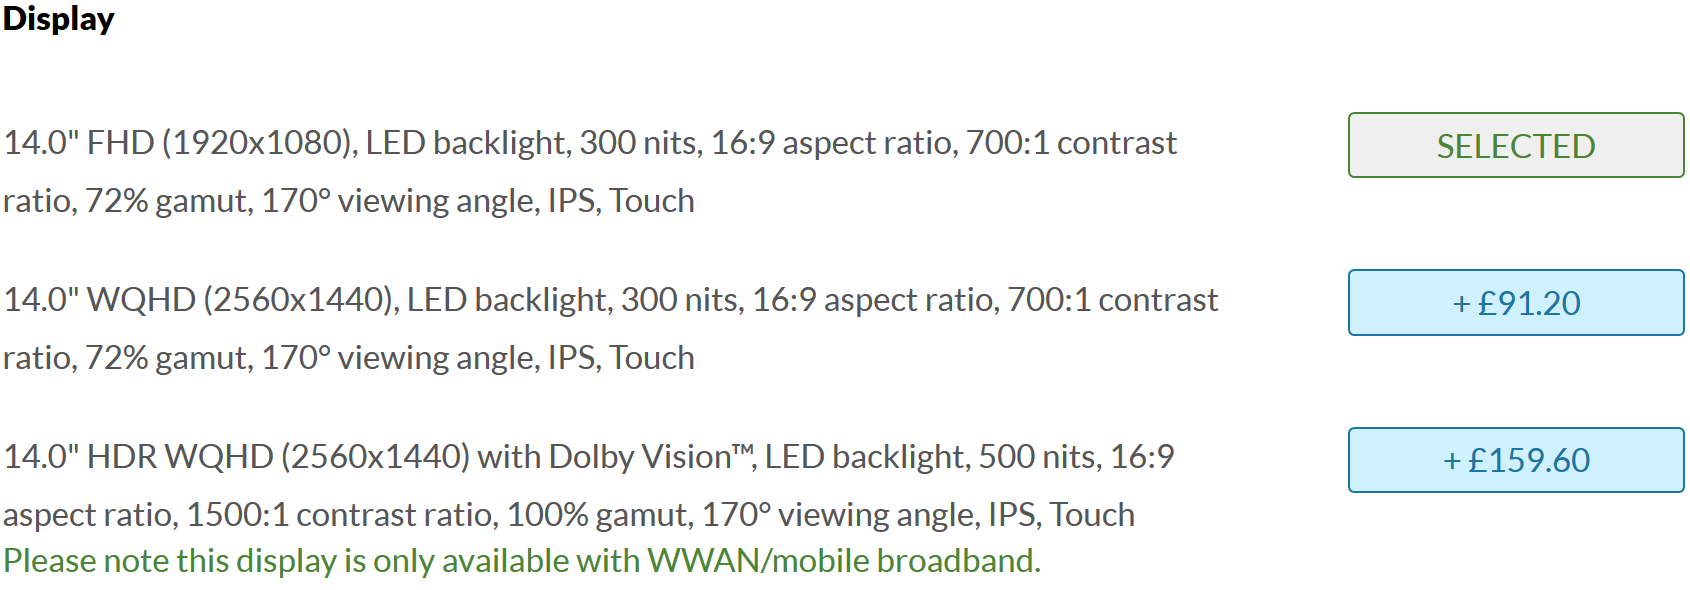
\includegraphics[width=\linewidth]{thinkpad-x1-yoga-display}}\only<2|handout:0>{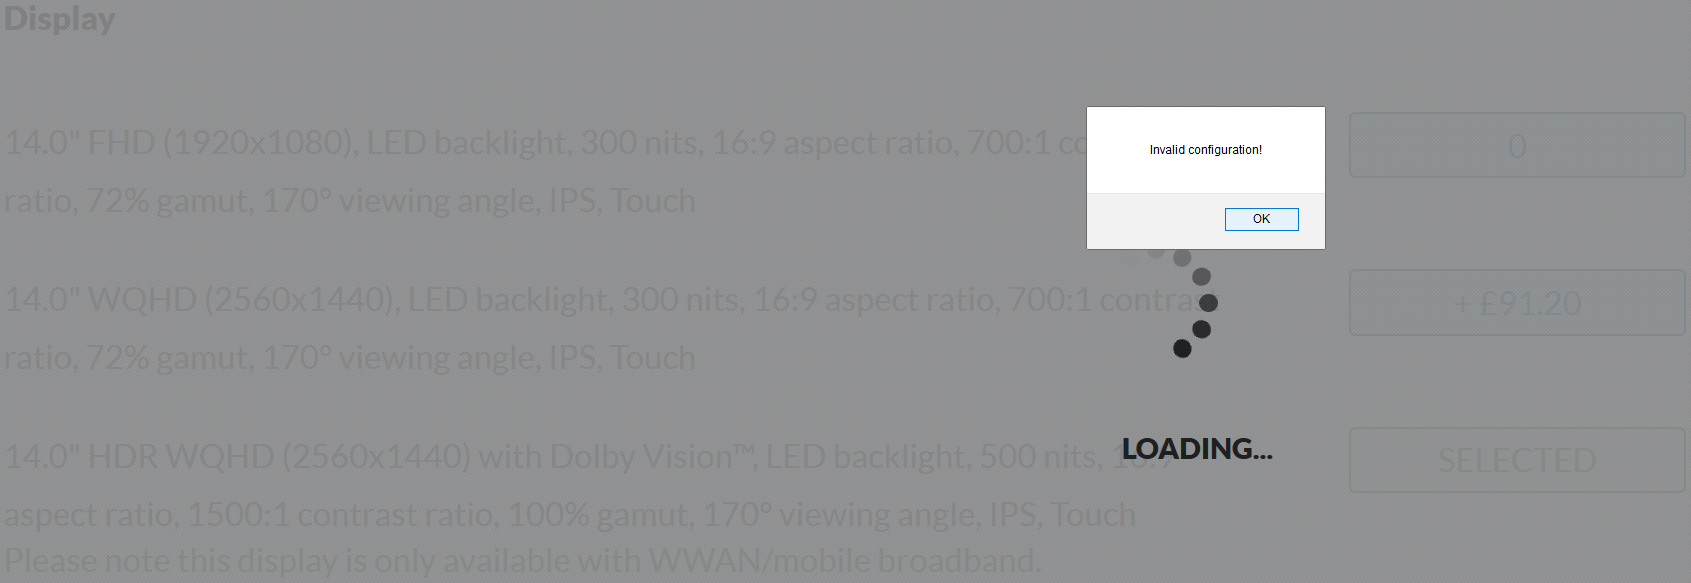
\includegraphics[width=\linewidth]{thinkpad-x1-yoga-display-invalidconf}}}}
\end{frame}

\begin{frame}{\insertsubsection}
	\partofpage{70}{\myexampletight{Still Configuring a Notebook}{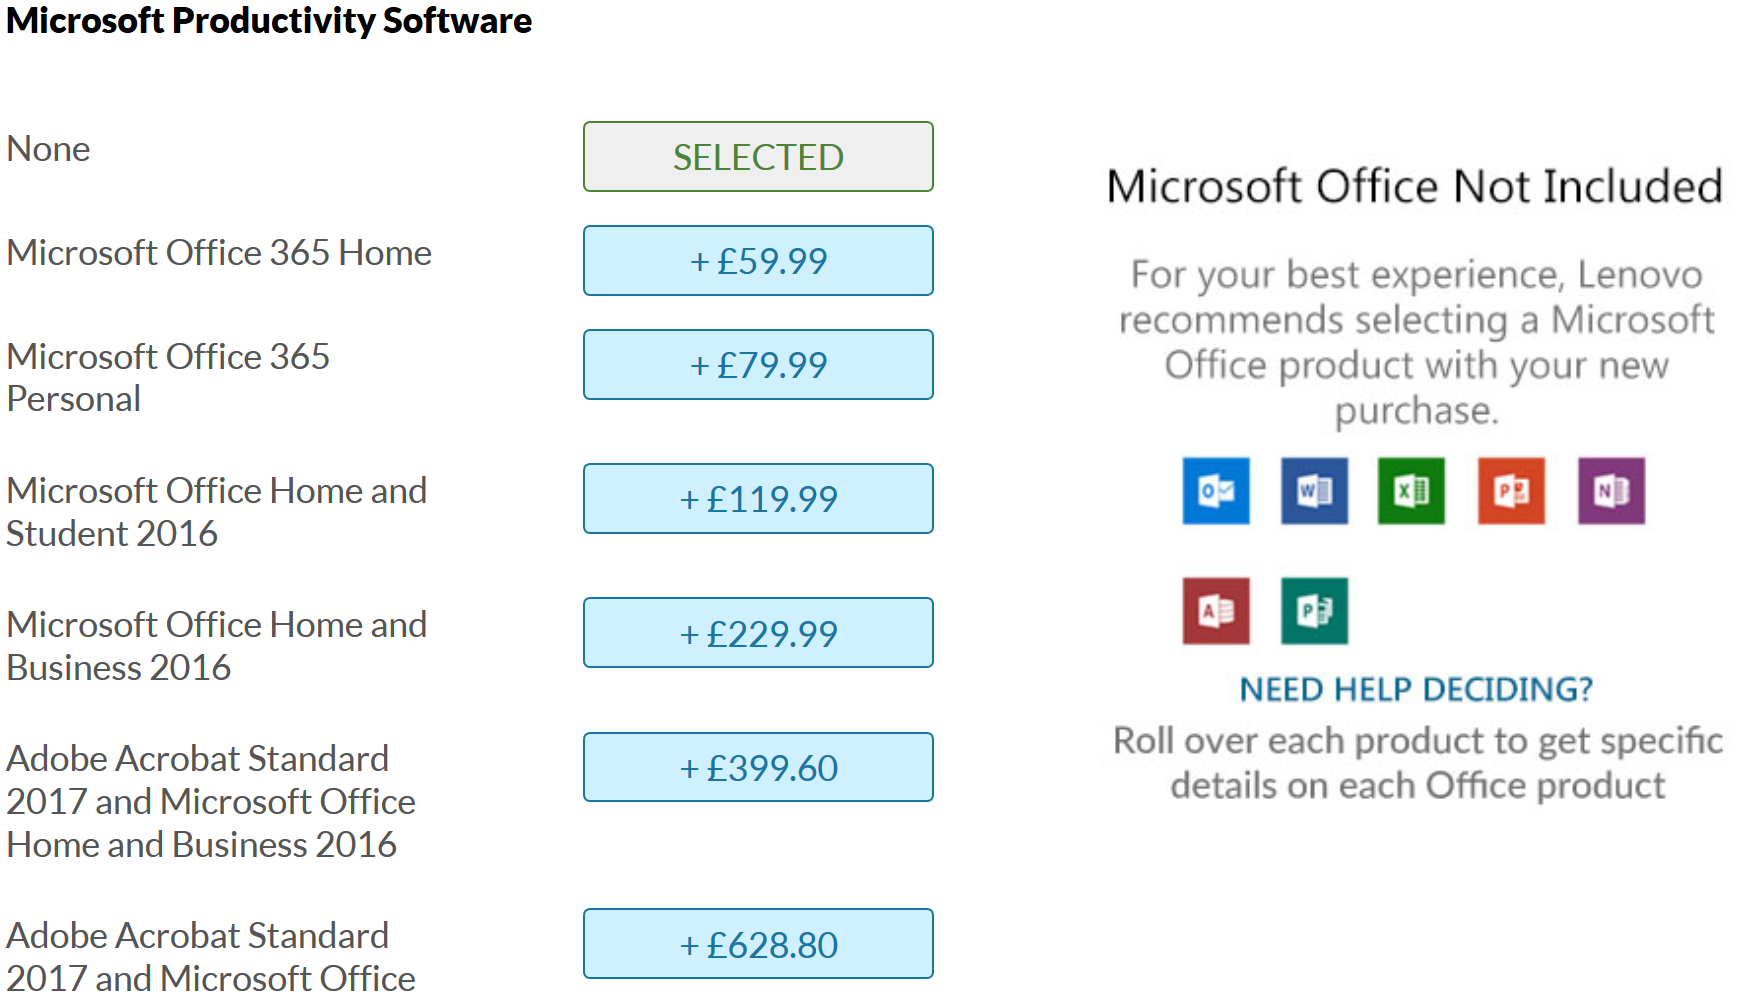
\includegraphics[width=\linewidth]{thinkpad-x1-yoga-office}}}
\end{frame}

\begin{frame}{\insertsubsection}
	~\hfill\partofpage{60}{\myexampletight{Configuring a Car}{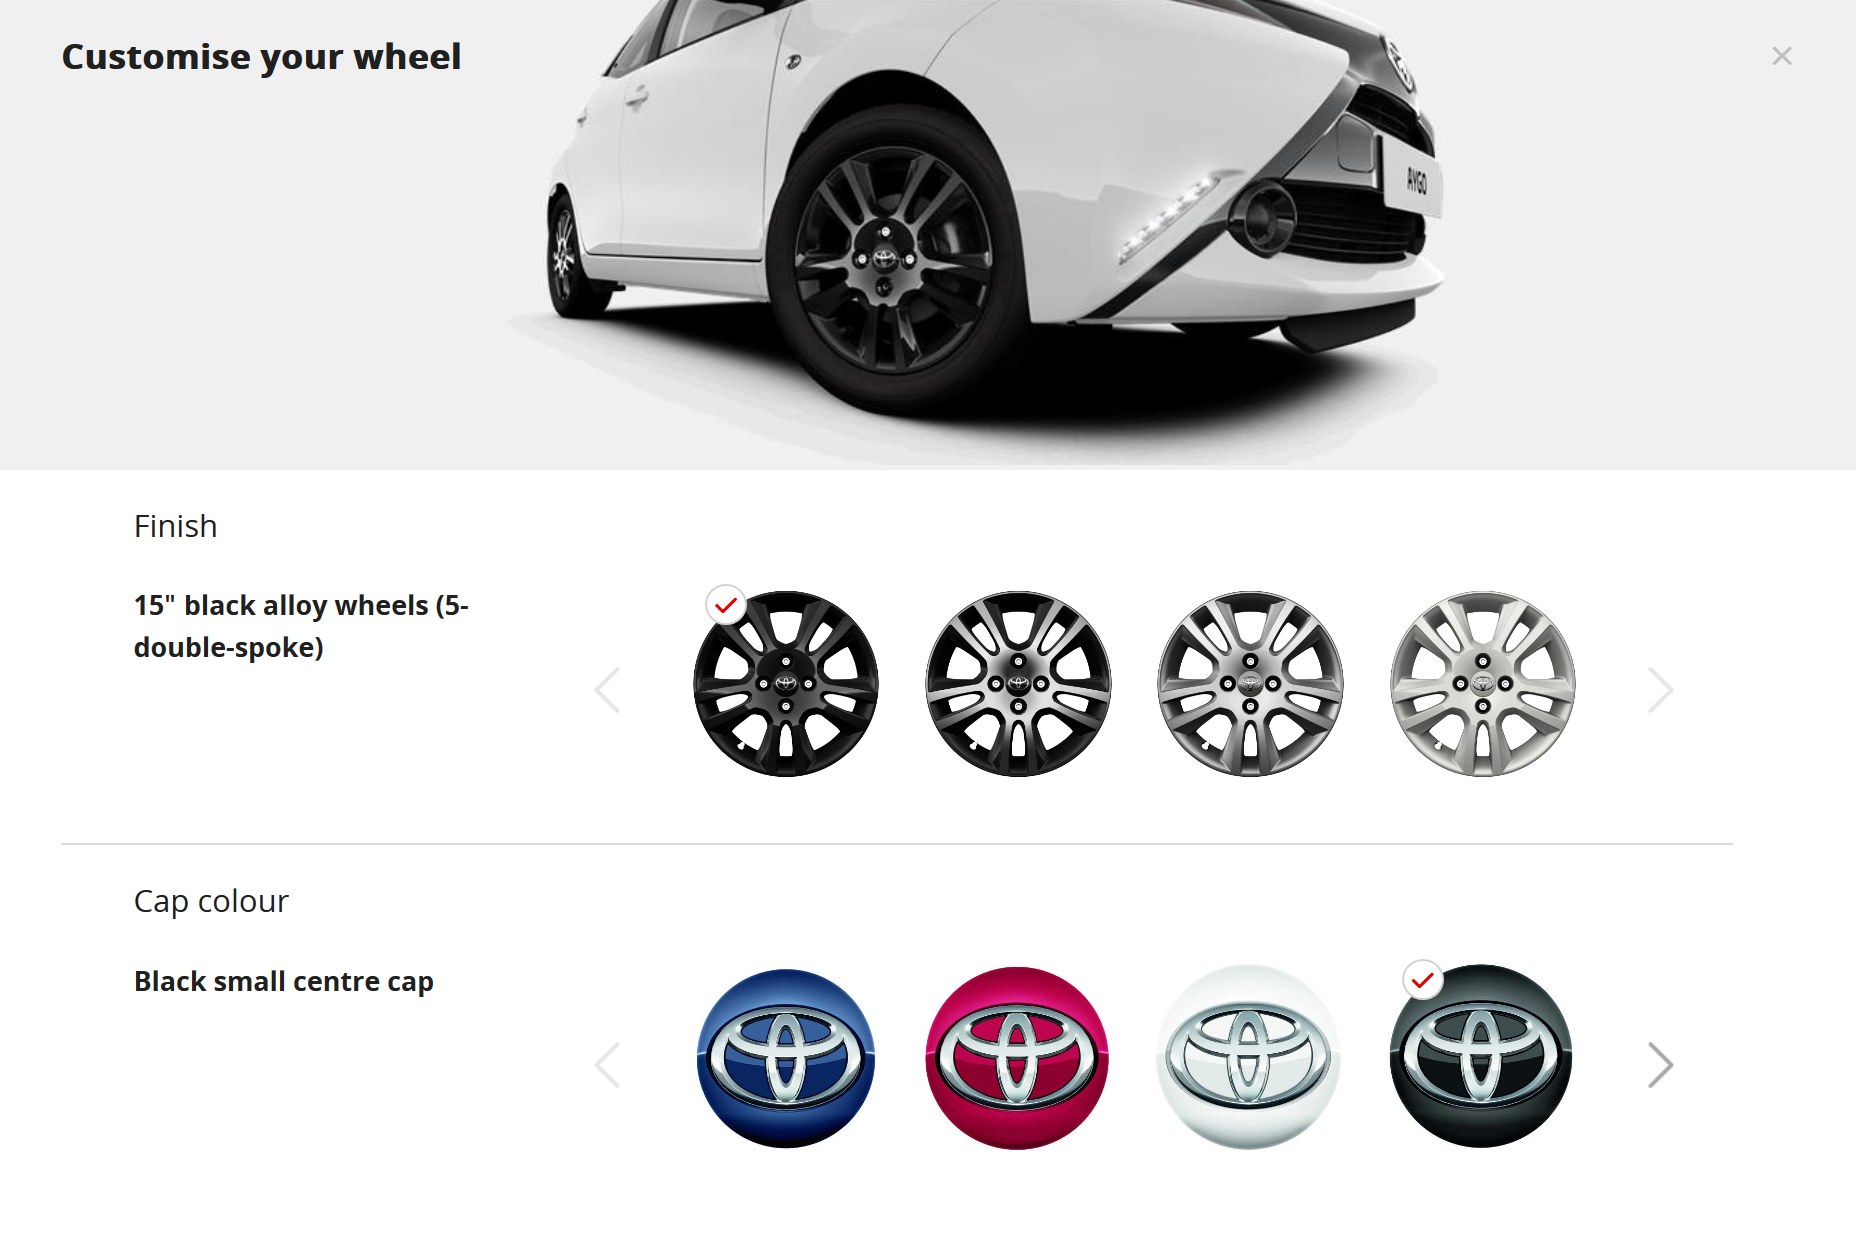
\includegraphics[width=\linewidth]{toyota-aygo-wheels}}}
\end{frame}

\begin{frame}{\insertsubsection}
	~\hfill\partofpage{60}{\myexampletight{Configuring a Car with a Weird Price}{\centering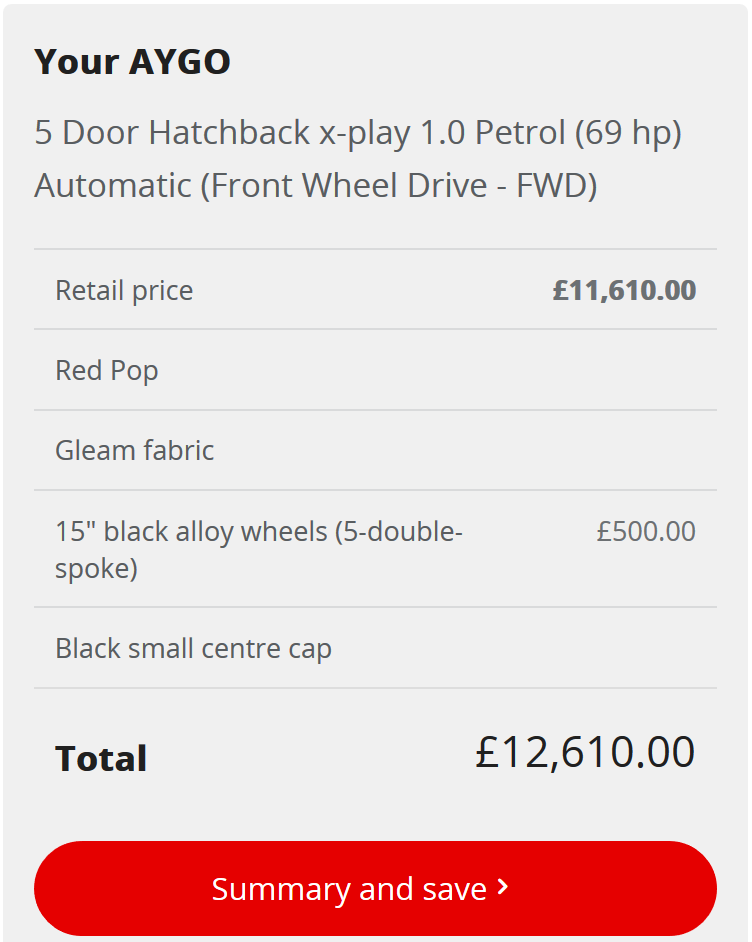
\includegraphics[width=.55\linewidth]{toyota-aygo-costs}}}
\end{frame}

\begin{frame}{\insertsubsection}
	~\hfill\partofpage{60}{\myexampletight{Configuring a Car with 8 Wheels!}{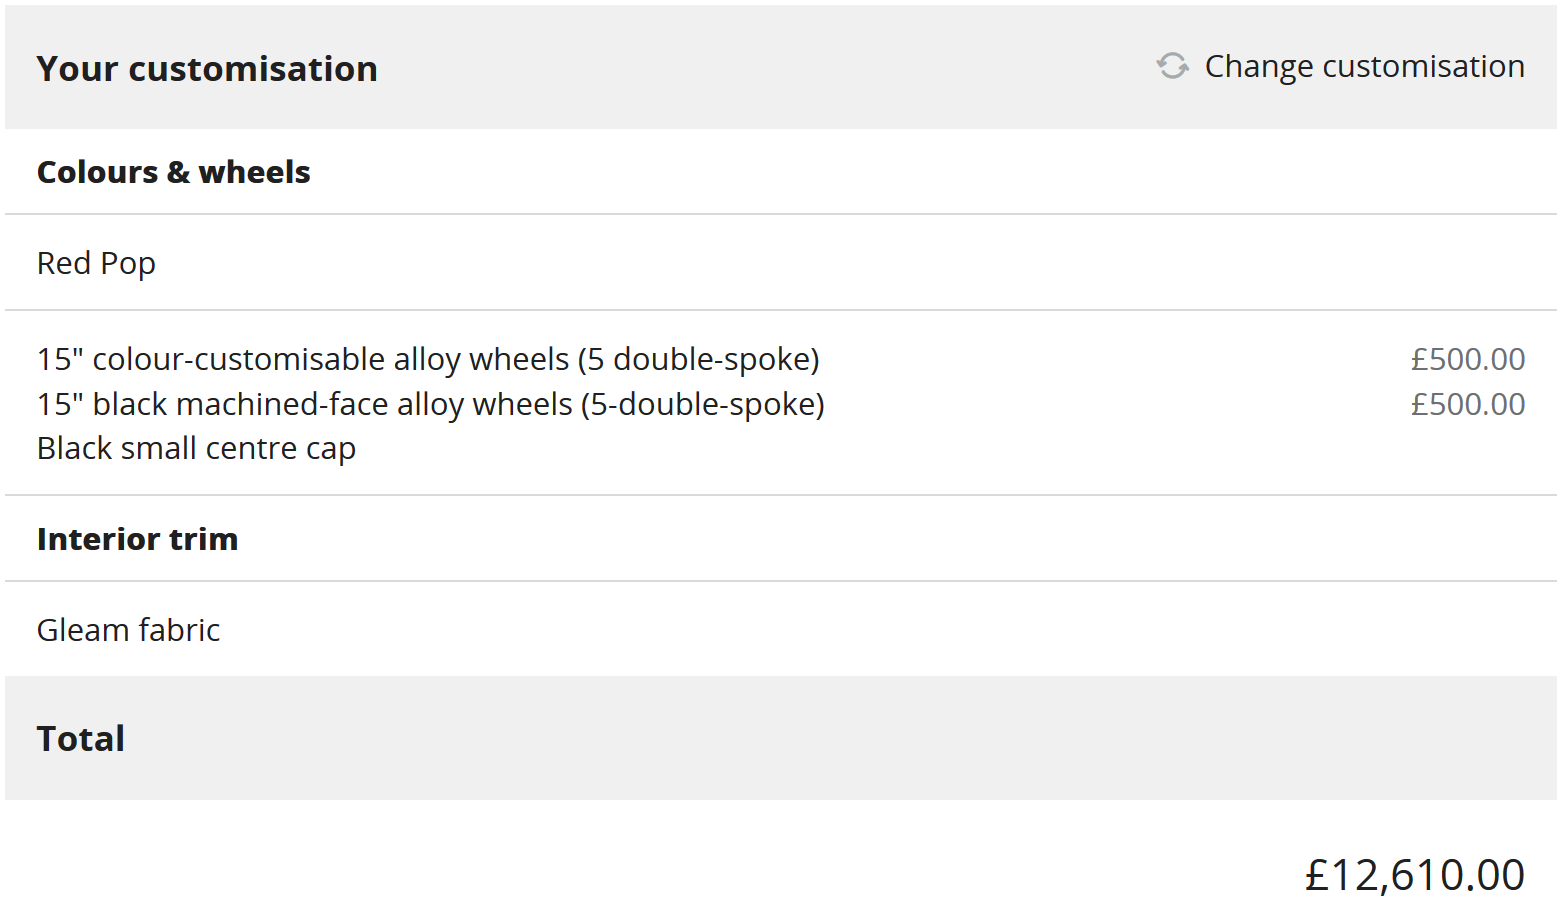
\includegraphics[width=\linewidth]{toyota-aygo-costs3}}}
\end{frame}

\begin{frame}{\insertsubsection}
	\partofpage{70}{\myexampletight{Configuring a German Car}{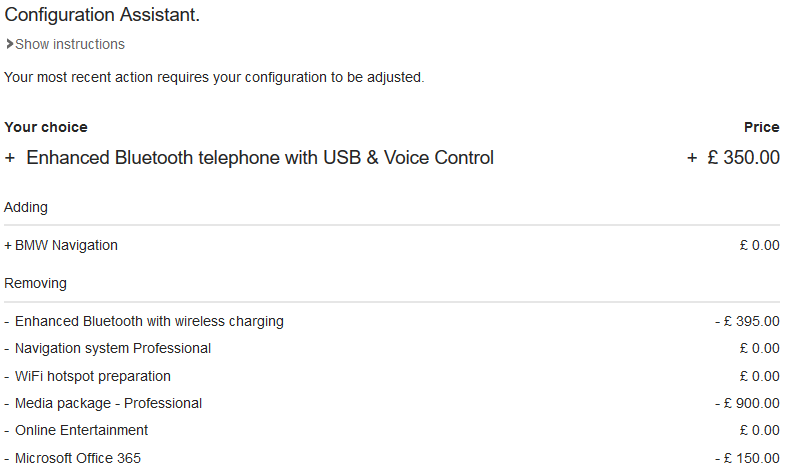
\includegraphics[width=\linewidth]{bmw-series1-confassistant-bluetooth}}}
\end{frame}

\subsection{Configurations}

\newcommand{\feat}[1]{{\emph{#1}}}

\begin{frame}{\insertsubsection}
	\leftorright{
		\mydefinition{Configuration}{
			\begin{itemize}
				\item a \emph{configuration} \deutsch{Konfiguration} over a set of features $F$ selects and deselects features in $F$
				\item formally: a pair $(S, D)$ such that $S, D \subseteq F$ and $S, D$ are disjoint ($S \cap D = \varnothing$)
				\item is \emph{complete} \deutsch{vollständig} if all features are covered ($S \cup D = F$) and \emph{partial} \deutsch{partiell} otherwise
				\item a complete configuration is \emph{valid} \deutsch{gültig} if it ``makes sense'' in the domain and \emph{invalid} \deutsch{ungültig} otherwise
    			\item we often abbreviate complete configurations with $S \equiv (S, F \setminus S)$
			\end{itemize}
		}
	}{
		\myexample{A Configurable Database}{
			Feature set $F = \{ConfigDB, Get, Put, Delete,$
			\hspace*{22mm}$Transactions, Windows, Linux\}$
			
			Examples for \emph{complete} configurations:
			\begin{itemize}
				\item \emph{Valid} (read-only database on Windows):
					$(\{C, G, W\}, \{P, D, T, L\})$
				\item \emph{Valid} (fully functional database on Linux):
					$(\{C, G, P, D, T, L\}, \{W\}\}$
				\item \emph{Invalid} ($\lightning$ no operating system):
					$(\{C, G\}, \{P, D, T, W, L\})$
				\item \emph{Invalid} (transactions $\lightning$ read-only database):
					$(\{C, G, T, L\}, \{P, D, W\})$
			\end{itemize}
			Examples for \emph{partial} configurations:
			
			$(\{C, G\}, \{P, D\})$, $(\varnothing, \varnothing)$, \ldots
		}
		
	}
\end{frame}

\subsection{Characterizing Valid Configurations}

\begin{frame}{\insertsubsection}\label{frame:natlang}
	\leftorright{
		\mynote{Valid Configuration}{
			A complete configuration over $F$ is valid if it ``makes sense'' in the domain.
			\emph{\color{red}{$\leadsto$ ``makes sense''?}}
		}

		\mydefinition{Natural Language}{
			\begin{itemize}
				\item informal description of relationships between features in $F$
				\item a complete configuration $S$ is \emph{valid} if it conforms to the description
    			\item[+] succinct
    			\item[--] sometimes ambiguous, not machine-readable
			\end{itemize}
		}
	}{
		\myexample{A Configurable Database}{
			``A \feat{configurable database} has an API that allows for at least one of the request types \feat{Get}, \feat{Put}, or \feat{Delete}.
			Optionally, the database can support \feat{transactions}, provided that the API allows for Put or Delete requests.
			Also, the database targets a supported operating system, which is either \feat{Windows} or \feat{Linux}.''
		}
	}
\end{frame}

\begin{frame}{\insertsubsection}\label{frame:cfgmap}
	\leftorright{
		\mynote{Valid Configuration}{
			A complete configuration over $F$ is valid if it ``makes sense'' in the domain.
			\emph{\color{red}{$\leadsto$ ``makes sense''?}}
		}

		\mydefinition{Configuration Map}{
			\begin{itemize}
				\item a \emph{configuration map} over $F$ is a set of complete configurations $C \subseteq F$
				\item a complete configuration $S$ is \emph{valid} if it occurs in the configuration map ($S \in C$)
				\item also known as product map
    			\item[+] precise
				\item[--] unreadable, redundant
				\item[--] explodes in size ($0 \leq \abs{C} \leq 2^{\abs{F}}$)
			\end{itemize}
		}
	}{
		\myexample{A Configurable Database}{
			Feature set $F = \{ConfigDB, Get, Put, Delete,$
			\hspace*{22mm}$Transactions, Windows, Linux\}$
			
			Configuration map:
			
			\small
			\leftandright{
				{\color{blue}$\{C,G,W\}$}\\
				$\{C,P,W\}$\\
				$\{C,G,P,W\}$\\
				$\{C,D,W\}$\\
				$\{C,G,D,W\}$\\
				$\{C,P,D,W\}$\\
				$\{C,G,P,D,W\}$\\
				$\{C,P,T,W\}$\\
				$\{C,G,P,T,W\}$\\
				$\{C,D,T,W\}$\\
				$\{C,G,D,T,W\}$\\
				$\{C,P,D,T,W\}$\\
				$\{C,G,P,D,T,W\}$
			}{
				$\{C,G,L\}$\\
				$\{C,P,L\}$\\
				$\{C,G,P,L\}$\\
				$\{C,D,L\}$\\
				$\{C,G,D,L\}$\\
				$\{C,P,D,L\}$\\
				$\{C,G,P,D,L\}$\\
				$\{C,P,T,L\}$\\
				$\{C,G,P,T,L\}$\\
				$\{C,D,T,L\}$\\
				$\{C,G,D,T,L\}$\\
				$\{C,P,D,T,L\}$\\
				{\color{blue}$\{C,G,P,D,T,L\}$}
			}
		}
	}
\end{frame}

\begin{frame}{\insertsubsection}
	\centering
	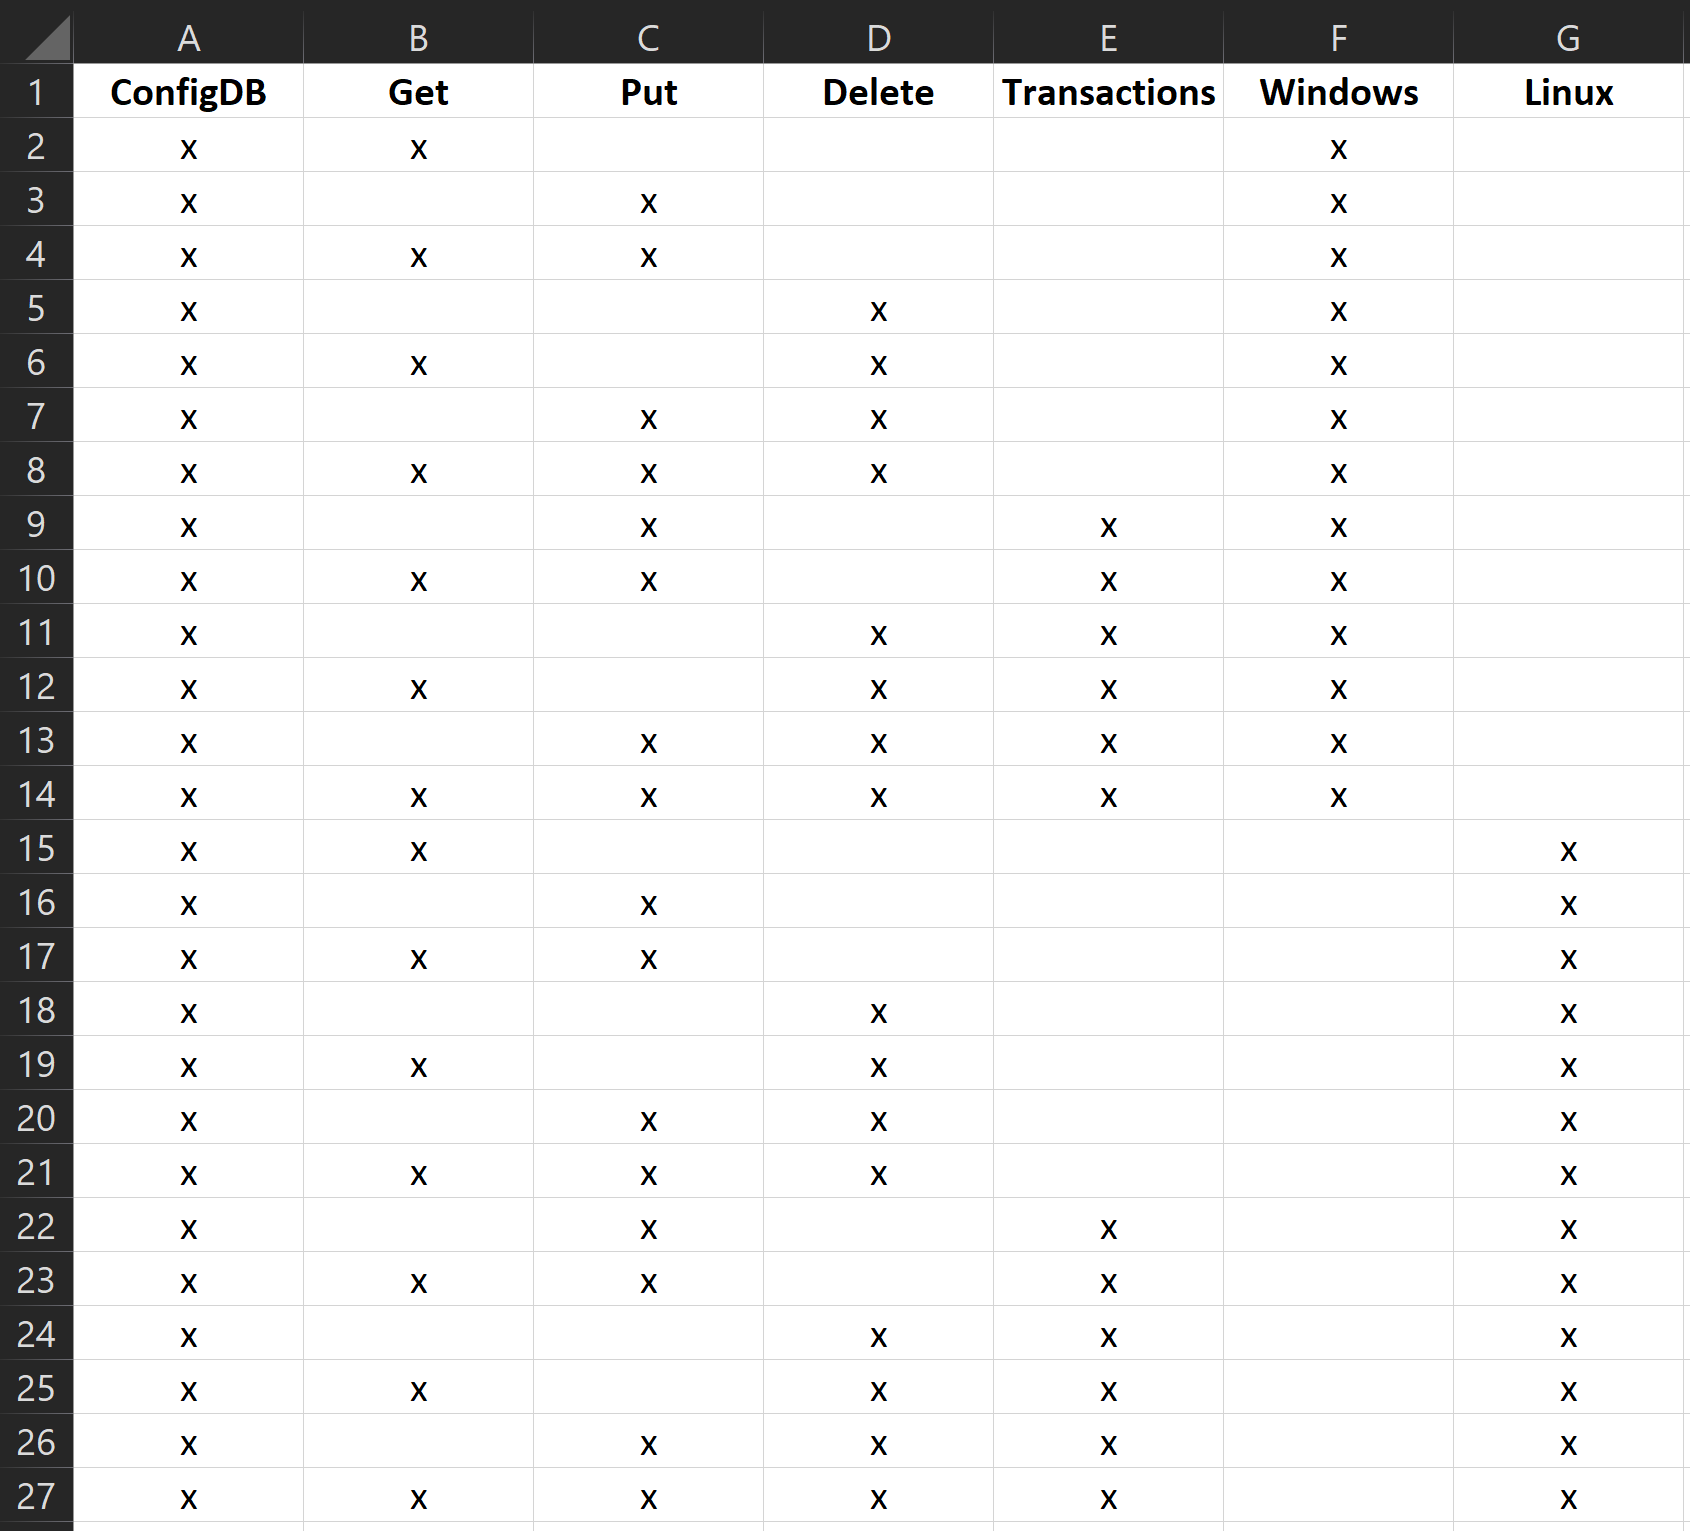
\includegraphics[width=0.48\linewidth]{products-in-excel}

	\textbf{Can we do better?}
\end{frame}

\subsection{Feature Models}

\newcommand{\dbmpl}{
	\myexampletight{A Configurable Database}{
		\centering
		\featureDiagramConfigurableDatabase

		\featureDiagramLegend
	}
}

\begin{frame}{\insertsubsection\ \mytitlesource{\fospl}}\label{frame:fm}
	\leftorright{
		\dbmpl
	}{
		\mydefinition{Feature Model \deutsch{Feature-Modell}}{
			\begin{itemize}
				\item hierarchy of features
				\item dependencies between features modeled by tree and cross-tree constraints
				\item \emph{tree constraints}: defined by the hierarchy
				\item \emph{cross-tree constraints}: propositional formulas over features
				\item \emph{abstract features} are used to group other features
				\item \emph{concrete features} have an implementation
    			\item also known as feature diagram or feature tree
			\end{itemize}
		}
	}
\end{frame}

\begin{frame}{\insertsubsection\ \mytitlesource{\fospl}}
	\leftorright{
		\dbmpl
	}{
		\mydefinition{Tree Constraints}{
			\begin{itemize}
				\item each feature requires its parent
				\item an \emph{optional feature} can be (de-)selected freely when its parent is selected
				\item a \emph{mandatory feature} is required by its parent
				\item \emph{or group}: at least one feature must be selected when the parent is selected
				\item \emph{alternative group}: exactly one feature must be selected when the parent is selected
			\end{itemize}
		}
		\mydefinition{Cross-Tree Constraints}{
			\begin{itemize}
				\item a list of propositional formulas expressing further dependencies between features
			\end{itemize}
		}
	}
\end{frame}

\begin{frame}{\insertsubsection\ \mytitlesource{\fospl}}
	\leftorright{
		\dbmpl
	}{
		\myexample{Valid Configurations \todo{animate}}{
			\begin{itemize}
				\item \emph{Valid} (read-only database on Windows):
					$(\{C, G, W\}, \{P, D, T, L\})$
				\item \emph{Valid} (fully functional database on Linux):
					$(\{C, G, P, D, T, L\}, \{W\}\}$
				\item \emph{Invalid} ($\lightning$ no operating system):
					$(\{C, G\}, \{P, D, T, W, L\})$
				\item \emph{Invalid} (transactions $\lightning$ read-only database):
					$(\{C, G, T, L\}, \{P, D, W\})$
			\end{itemize}
			
		}
	}
\end{frame}

\begin{frame}{\insertsubsection\ \mytitlesource{\fospl}}
	\leftorright{
		\todo{other feature diagram example(s) which shows off how notation can also be used}
		% graph product line example?
	}{
		\mynote{Notation}{
			\begin{itemize}
				\item abstract and concrete features can be assigned arbitrarily
    			\item groups can be used anywhere
				\item directly below groups, no optional or mandatory markers are allowed
			\end{itemize}
		}
	}
\end{frame}

\subsection{Advantages of Feature Modeling}
\begin{frame}{\insertsubsection}
	\leftandright{
		\textbf{Making Tacit Knowledge Explicit}
		\mynote{Interview with Practitioners \mysource{\href{https://link.springer.com/chapter/10.1007/978-3-319-11653-2_19}{Berger~et~al.~2014}}}{
			\mycite{I think the best [about feature modeling] is you can see relationships, to actually know what configurations are allowed and what are not allowed. That was also not so easy to express in the past [\ldots] This is from the developer’s point of view. But it’s also, we can see that from the, say project development, it’s also important, because before we noticed that \emph{the same functionality was implemented twice} within the same project, basically they haven’t realized that. They implemented the same features.}
		}
	}{
		\textbf{Tool Support}

		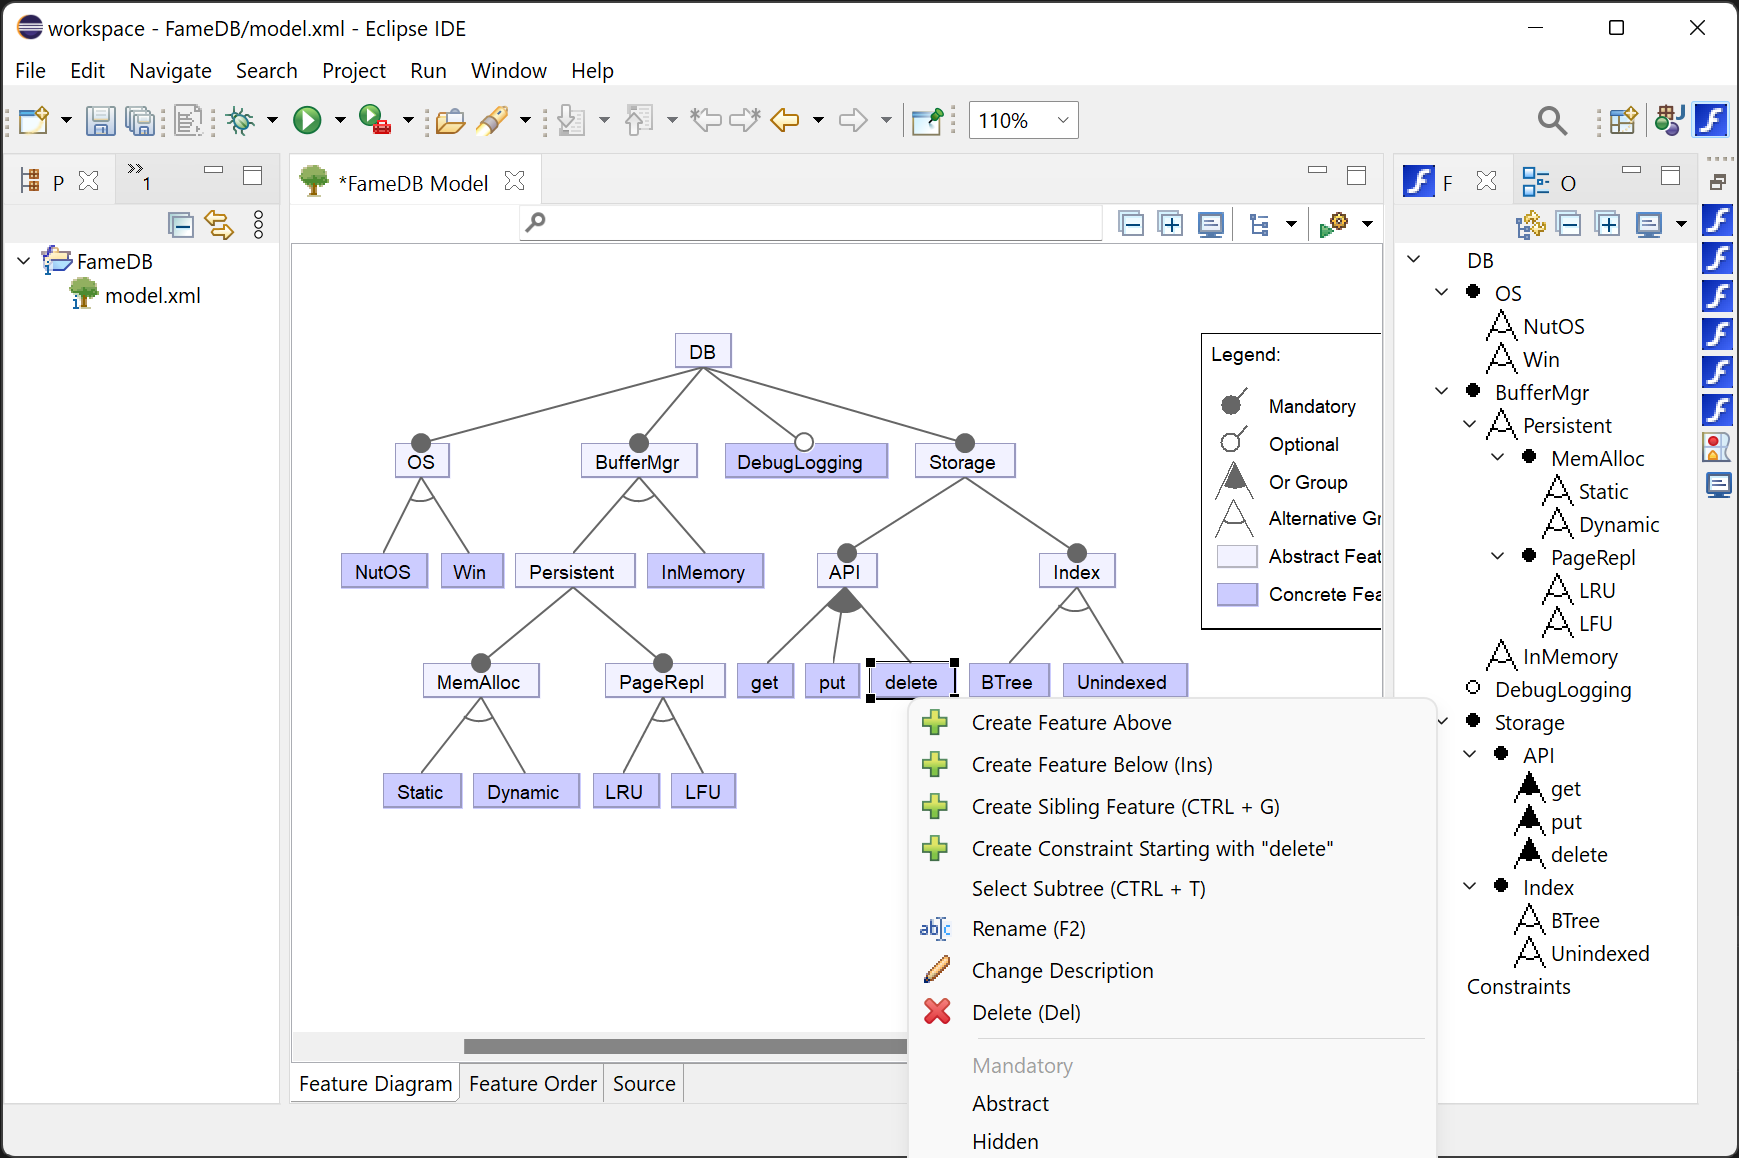
\includegraphics[width=\linewidth]{featureide-feature-model-editor}
	}
\end{frame}

% advantages over Natural Language, List of Configurations

\lessonslearned{
	\item Features, dependencies between features, configurators
	\item Feature models: abstract and concrete features, tree and cross-tree constraints
	\item Tree constraints: optional, mandatory, or group, alternative group
}{
	\item \fospl, Section~2.3 Feature Modeling
	\item Thorsten Berger et al. (2013): \href{https://doi.org/10.1145/2430502.2430513}{A Survey of Variability Modeling in Industrial Practice}
	\item Damir Nešić et al. (2019): \href{https://doi.org/10.1145/3338906.3338974}{Principles of Feature Modeling}
}{
	% \item In the feature model below, is the configuration $\{Base, API, Put, Trans., Win\}$ valid? % no, root+OS missing % block 3?
	% \featureDiagramConfigurableDatabase

	% $\mathit{Transactions} \pimplies \mathit{Put} \por \mathit{Delete}$
	\item Sketch a feature model with X configurations (pen and paper preferred)
    \item Upload your solution to ...
    \item Discuss whether your solutions are syntactically correct
	% \item Sketch a feature model that has 9 valid configurations (pen and paper preferred)
 	% \item Discuss whether your solutions are syntactically correct and have the right number of configurations
}

%block 1: features explizit + ihre abhängigkeiten auch 
%notation für modell nutzen + eins zeichnen mit mind. 5 features, fehler korrigieren, lesen von modellen üben

\sectionend

% second: semantics of feature diagrams and other modeling notations (how can we encode features machine-readably?)
\section{Representations and Translations}

\subsection{Representations of Variability Models}

\begin{frame}{\insertsubsection} % show list of cfgs, diagrams, text => what are the problems? 
	% this notation is already nice for communication, but semantics matter (for large models, it does not suffice to look sharply)

	% why is this needed? (forward ref?)

	% this section shall teach the relationship between FMs and formulas and FMs and sets (i.e., Damiani 2020, Batory 2005), so: FM semantics

	% also, (valid) total configurations should be explained here (how a computer can check them, this can be checked easily when an FM is encoded eg as runtime variability, but all other SAT-based questions are hard to answer)

	% recount the example model here

	\leftandright{
		\myexample{Natural Language}{
			\tiny ``A \feat{configurable database} has an API that allows for at least one of the request types \feat{Get}, \feat{Put}, or \feat{Delete}.
			Optionally, the database can support \feat{transactions}, provided that the API allows for Put or Delete requests.
			Also, the database targets a supported operating system, which is either \feat{Windows} or \feat{Linux}.''
		}
		\myexample{Configuration Map}{
			\tiny
			\leftandright{
				$\{C,G,W\}$\\
				\hspace{4mm}\vdots\\[1ex]
				$\{C,G,P,D,T,W\}$
			}{
				$\{C,G,L\}$\\
				\hspace{4mm}\vdots\\[1ex]
				$\{C,G,P,D,T,L\}$
			}
		}
		\myexampletight{Feature Model}{
			\centering\tiny
			\featureDiagramConfigurableDatabase
		}
	}{
		\centering
		\usetikzlibrary{positioning}
		\begin{tikzpicture}
			\tikzstyle{every edge}=[font=\tiny,draw,color=blue]
	
			\node (fd) at (2,0) [align=center] {Feature Model\\[-1ex]\tiny\refslide{frame:fm}\\[-1ex]{\tiny\color{red}P1}};
			\node (nat) at (0,-2) [align=center] {Natural Language\\[-1ex]\tiny\refslide{frame:natlang}\\[-1ex]{\tiny\color{red}TXT, RTF}};
			\node (cfg) at (4,-2) [align=center] {Configuration Map\\[-1ex]\tiny\refslide{frame:cfgmap}\\[-1ex]{\tiny\color{red}CSV, XLS}};
	
			\path [->] (fd) edge[bend left] node[sloped,yshift=1mm] {toString} (nat);
			\path [dotted, ->] (nat) edge[bend left] node[sloped,yshift=1mm] {P3} (fd);
			
			\path [dotted, ->] (fd) edge[bend left] node[sloped,yshift=1mm] {P2} (cfg);
			\path [dotted, ->] (cfg) edge[bend left] node[sloped,yshift=1mm] {P3} (fd);

			\node (trans) at (-1,-2.8) {};
			\node (trans2) at (2,-2.8) {};
			\node (trans3) at (-1,-3.1) {};
			\node (trans4) at (2,-3.1) {};
			\path [->] (trans) edge node[yshift=1mm] {automated transformation} (trans2);
			\path [dotted, ->] (trans3) edge[yshift=5mm] node[yshift=1mm] {semi-automated transformation} (trans4);
		\end{tikzpicture}

		\mynote{Problems}{
			\begin{enumerate}%[label=P\arabic*]
				\item How to express feature models textually?
				\item How to obtain configurations automatically?
    			\item \color{gray}{(How to reverse engineer feature models?)}
			\end{enumerate}
		}
	}
\end{frame}


\subsection{Universal Variability Language}

\begin{frame}{\insertsubsection}
	\leftorright{
		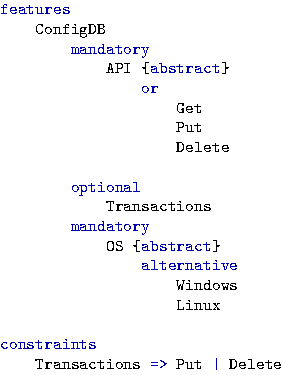
\includegraphics[width=0.7\linewidth]{uvl-model}
	}{
		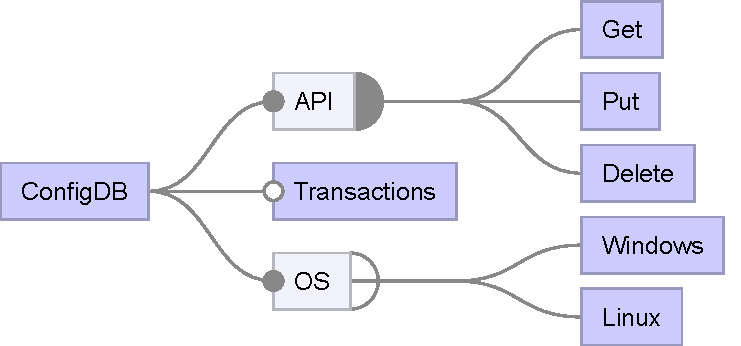
\includegraphics[width=\linewidth]{varied-model}
		\mynote{UVL}{
			\begin{itemize}
				\item textual language for feature modeling
    			\item 
			\end{itemize}
		}
	}
\end{frame}

% \subsection{List of Valid Configurations}

% \begin{frame}{\insertsubsection}
% 	what is a (valid) configuration? define as a set of selected features (only later extend to partial configurations)

% 	this is basically an Excel sheet

% 	first explain product lists / sets and configuration validity (ie, set membership): (use same example)

% 	$ext-sem (FM) = \{ C \mid C in 2^F | C satisfies all FM rules \}$

% 	this is a nice (readable) semantics (directly connected to relational databases) but impractical to check, so we need formulas as a concise representation
% \end{frame}

\subsection{Propositional Formulas}

\begin{frame}{\insertsubsection}
	Syntax of formulas

	explain $\pand, \por, \pnot, \pimplies, \pequals$

	here, we do not allow $\forall, \exists$ (extensions exist: QBF (e.g., slicing), FOL (non-Boolean models))
\end{frame}

\begin{frame}{\insertsubsection}
	show running example as a formula
	
	explain intuition behind elements of formula

	motivate very shortly why this might be nice

	there is evidence (Knueppel) that the full expressive power of Boolean formulas is needed for real-world formulas
\end{frame}

\subsection{From Diagram to Formula}

\begin{frame}{-- Algorithm}
	formal algorithm for transformation into FOL (and then CNF?)
\end{frame}

\subsection{Canonical Formula Representation(s?)}

\begin{frame}{-- Conjunctive Normal Form}
	CNF is a universal language for saving Boolean formulas, maybe explain it here?
\end{frame}

\begin{frame}{-- Equivalent Transformation}
	
\end{frame}

\begin{frame}{-- DIMACS File Format}
	
\end{frame}

%(state BDD?)
% probably not - (knowledge compilation: there are many nuances between CNF and BDD, maybe discuss?)

\subsection{Other Representations} %variations? these are not only other representations of the same notation

\begin{frame}{\insertsubsection}
	Extended Feature Models
	
	%at the end (what else is there?): in practice, we also have non-Boolean features/attributes/constraints over attributes (more details on efficiency in third block)

	Cardinalities

	Linux/Kconfig % tri-state features
\end{frame}







% \subsection{Enumerating All Configurations}
% \begin{frame}{\insertsubsection}
% 	\leftandright{
% 		%\myexampletight{}{\centering\includegraphics[width=.75\textwidth]{db-constraint}}
% 		\myexample{26 Valid Configurations}{
% 			\footnotesize
% 			\leftandright{
% 				$\{B,G,W\}$\\
% 				$\{B,P,W\}$\\
% 				$\{B,G,P,W\}$\\
% 				$\{B,D,W\}$\\
% 				$\{B,G,D,W\}$\\
% 				$\{B,P,D,W\}$\\
% 				$\{B,G,P,D,W\}$\\
% 				$\{B,P,T,W\}$\\
% 				$\{B,G,P,T,W\}$\\
% 				$\{B,D,T,W\}$\\
% 				$\{B,G,D,T,W\}$\\
% 				$\{B,P,D,T,W\}$\\
% 				$\{B,G,P,D,T,W\}$
% 			}{
% 				$\{B,G,U\}$\\
% 				$\{B,P,U\}$\\
% 				$\{B,G,P,U\}$\\
% 				$\{B,D,U\}$\\
% 				$\{B,G,D,U\}$\\
% 				$\{B,P,D,U\}$\\
% 				$\{B,G,P,D,U\}$\\
% 				$\{B,P,T,U\}$\\
% 				$\{B,G,P,T,U\}$\\
% 				$\{B,D,T,U\}$\\
% 				$\{B,G,D,T,U\}$\\
% 				$\{B,P,D,T,U\}$\\
% 				$\{B,G,P,D,T,U\}$
% 			}
% 		}
% 	}{}
% \end{frame}

% \subsection{Linux Feature Model}
% \begin{frame}{\insertsubsection}
% 	\vspace{28mm}~\hspace{-15mm}\href{https://dl.acm.org/doi/abs/10.1145/3382025.3414943}{\includegraphics[width=1.2\linewidth,trim=100 510 100 170,clip]{linux-bdd}}
% \end{frame}

% \subsection{Dependencies Modeled in Excel}
% \begin{frame}{\insertsubsection}
% 	\vspace{-7mm}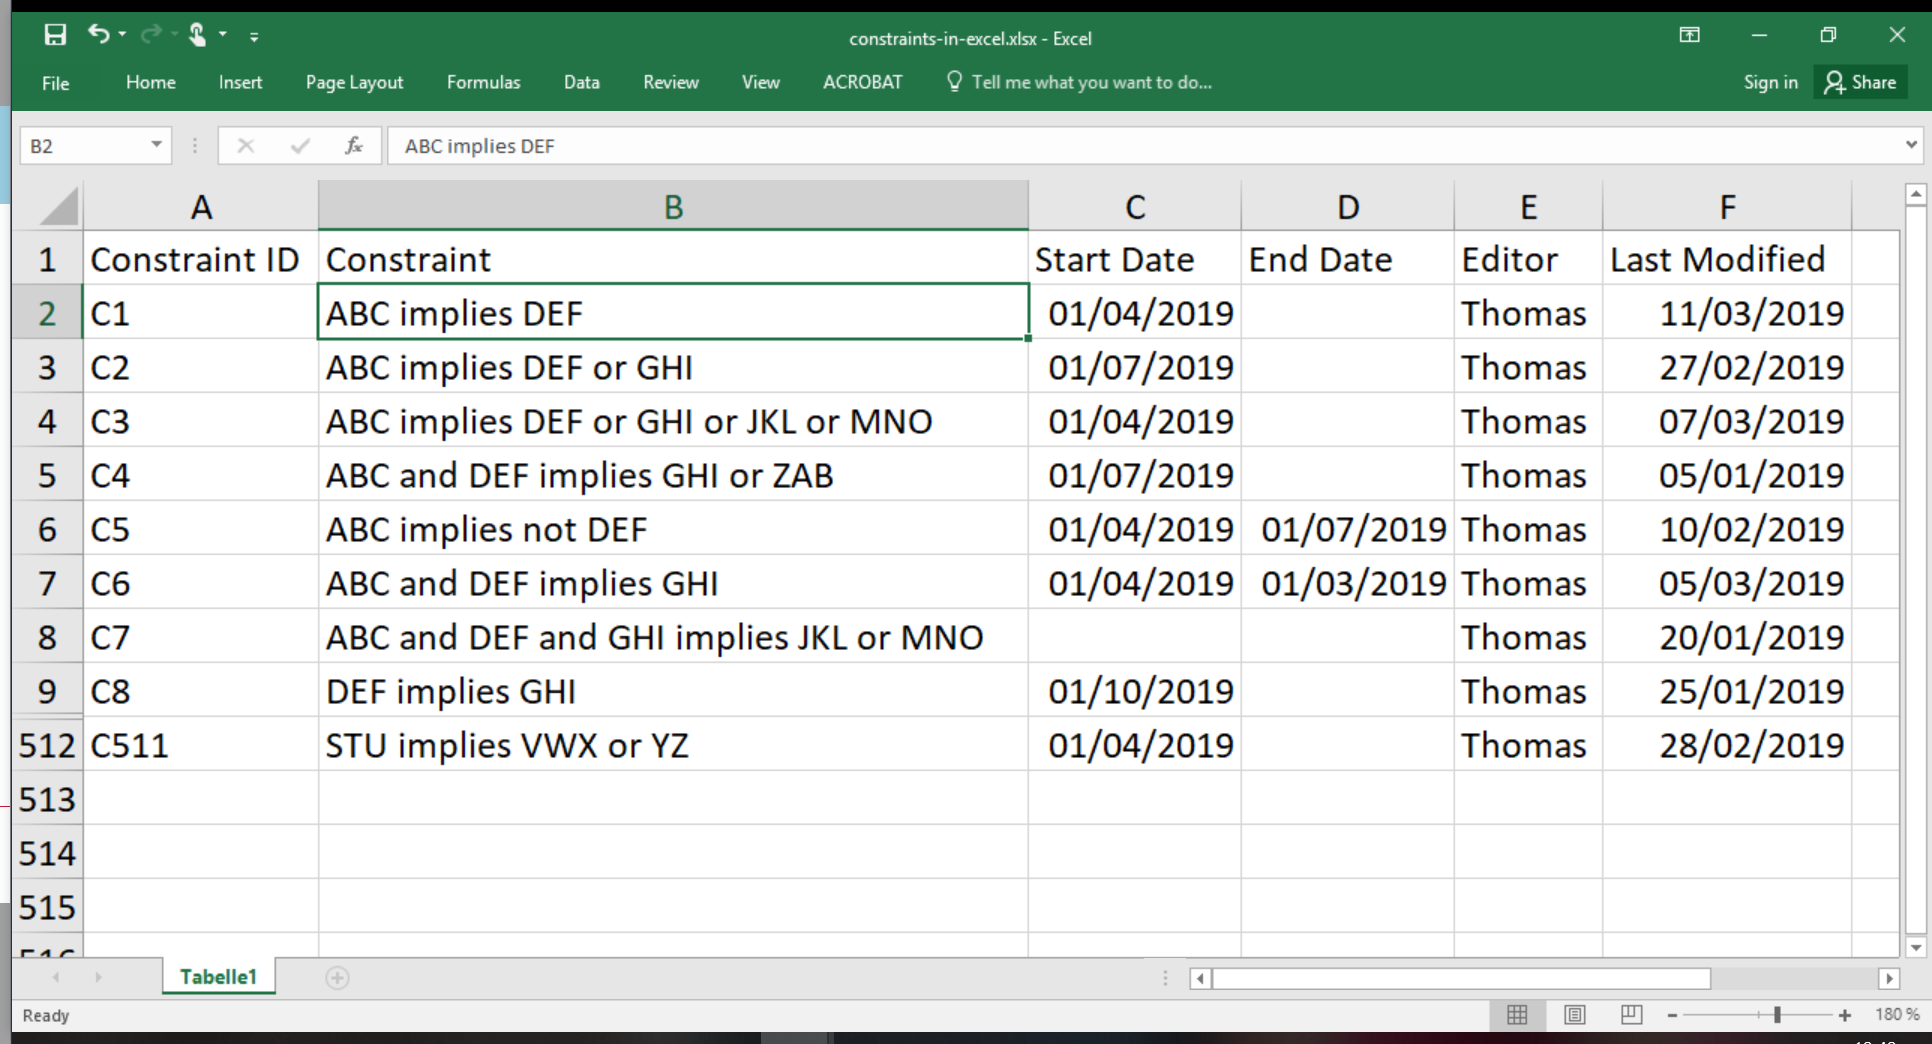
\includegraphics[width=.7\linewidth,trim=10 10 0 10,clip]{constraints-in-excel}
% \end{frame}

\begin{frame}{\insertsubsection}
	\myexampletight{Representations of Variability Models}{
		\usetikzlibrary{positioning}
		\begin{tikzpicture}
			\tikzstyle{every edge}=[font=\tiny,draw,color=blue]
	
			\node (topleft) at (-1,0) {};
			\node (bottomleft) at (-1,-4) {};
			\node (bottomleft2) at (-0.5,-4) {\tiny\color{red}File Format};
			
			\node (fd) at (2,0) {Feature Model};
			\node (fd2) at (fd.south) {\tiny\color{red}UVL, XML};
			\node (nat) at (0,-2) [align=center] {Natural\\Language};
			\node (nat2) at (nat.south) {\tiny\color{red}Plain/Rich Text};
			\node (phi) at (2,-2) [align=center] {Propositional\\Formula};
			\node (phi2) at (phi.south) {\tiny\color{red}Excel, SMT-LIB};
			\node (cfg) at (4,-4) {Product Map};
			\node (cfg2) at (cfg.south) {\tiny\color{red}Excel, CSV};
			\node (cnf) at (2,-4) {CNF};
			\node (cnf2) at (cnf.south) {\tiny\color{red}DIMACS};
	
			\path [dotted, thick, ->] (topleft) edge node[left, rotate=90, yshift=2mm, xshift=10mm] {Loss of Structure} (bottomleft);
		
			\path [->] (fd2.south west) edge[bend left=15] node[sloped,yshift=1mm] {see slide X} (nat);
			\path [dashed, ->] (nat) edge[bend left=15] node[sloped,yshift=1mm] {\footnote{\bakarnaturallanguage}} (fd2.south west);
			
			\path [->] (fd2.south) edge[bend left=15] node[sloped,yshift=1mm] {see slide X} (phi);
			\path [dashed, ->] (phi) edge[bend left=15] node[sloped,yshift=1mm] {\footnote{\czarneckithereandbackagain, \shereverseengineering}} (fd2.south);

			\path [dashed, ->] (fd2.south east) edge[bend left=8] node[sloped,yshift=1mm] {see slide X} (cfg);
			\path [dashed, ->] (cfg) edge[bend left=8] node[sloped,yshift=1mm] {\todots} (fd2.south east);

			\path [->] (phi2) edge[bend left=15] node[sloped,yshift=1mm] {see slide X} (cnf);
			\path [dashed, ->] (cnf) edge[bend left=15] node[sloped,yshift=1mm] {\todots} (phi2);
		
			\path [dashed, ->] (cfg) edge[bend right=15] node[sloped,yshift=1mm] {see slide X} (cnf);
			\path [dashed, ->] (cnf2.south) edge[bend right=15] node[sloped,yshift=1mm] {AllSAT} (cfg2);
		\end{tikzpicture}
	}
\end{frame}

\lessonslearned{
	\item To understand large configuration spaces, formal semantics and machine-readable representations matter.
	\item Propositional formulas satisfy many (though not all) needs for such a representation.
}{
	\item Don Batory (2005): \href{https://doi.org/10.1007/11554844_3}{Feature Models, Grammars, and Propositional Formulas}
	\item Alexander Knüppel et al. (2017): \href{https://doi.org/10.1145/3106237.3106252}{Is There a Mismatch Between Real-World Feature Models and Product-Line Research?}
}{
	\item Figure out how many valid configurations your feature diagram represents.
	When is this easy?
	\item Translate (a part of) your feature diagram into a formula, then into CNF, and finally into a DIMACS file.
	How might this be useful?
}
% translate your model into a propositional formula
%block 2: formel hinschreiben, valide + invalide cfg aufschreiben

\sectionend

% third: analyses of feature models (what can a computer tell us, which we cannot tell just by looking?)
\section{Automated Analyses}

\subsection{Asking Questions About Feature Models}

% do everything with one running example (preferably the one from before)
% ie, show an example of an inconsistency and then reveal the issue - can be combined with the MUS explanations

\begin{frame}{\insertsubsection}
	this section should teach all usual FM/cfg analyses - some in more detail, some only high-level (other SPL analyses come in analyses.tex)

	list questions we might want to ask a feature model (maybe grouped in the order in which they are discussed)

	include some simple \#SAT questions (e.g., feature prioritization)

	am i developing unused code?

	how to find out whether a partial configuration is valid? (show decision propagation in FeatureIDE)

	etc.
\end{frame}

\subsection{Automated Reasoning with SAT and \#SAT}

\begin{frame}{-- Problem}
	recapitulate (very basic) theory behind both problems

	revisit what the class of programs named "solver" does, and why it is important that we use OTS solvers and profit from their optimizations/contests - idea: reduce practical problems to solvers (sim. to TheoInf/Logics)
\end{frame}

%sat, taut

\begin{frame}{-- Solvers}
	explain simple SAT and \#SAT solver ($SAT(\phi) \in \{\top, \bot\}$)

	as a black-box/abstraction (may be implemented in many ways, e.g. as BDD)

	extensions to SAT solver interface (harder to implement):
	
	when SAT = true, some give a satisfying assignment (for optimizations)
	
	wen SAT = false, some give a MUS (for explanations) % see master theses of T. Günther, S. Ananieva

	\#SAT subsumes SAT, but is harder to compute
\end{frame}

\subsection{Void Feature Model}
\begin{frame}{\insertsubsection}
	is the FM even consistent? does it have errors? % can we even get a valid configuration? does a configurator allow anything? a clever configurator would see that

	void iff $SAT(\phi) = \bot$

	for each analysis, also list \#SAT encoding
	to WHICH DEGREE is a FM consistent (i.e., degree of freedom / variability factor)?

	also list explanations / MUS (very shortly)

	maybe for each analysis, list applications/scenarios, here: find grave modeling errors, check wether a configurator even allows to create ANY valid configuration
\end{frame}

\subsection{Core and Dead Features} % + these are variability smells
\begin{frame}{\insertsubsection}
	can a feature be chosen at all? is it false-optional?
	to WHICH DEGREE is a feature core/dead? feature prioritization

	f core iff $SAT(\phi and not f) = \bot$
	
	f dead iff $SAT(\phi and f) = \bot$

	applications: find anomalies/inconsistencies (false-optional), commonality, feature prioritization
\end{frame}

\subsection{Partial Configurations}
\begin{frame}{\insertsubsection}
	can a partial configuration be completed?
	can also be connected to Chico's \#SAT applications

	note that this is a generalization of void/core/dead

	total configurations were defined before, now expand this definition to a tuple $(sel, desel)$ and explain why

	applications: ...
\end{frame}

\subsection{Redundant Constraints (?)}
\begin{frame}{\insertsubsection}
	... % include this? it has no real #SAT equivalent
\end{frame}

\subsection{Other Analyses}
\begin{frame}{\insertsubsection}
	list some more analyses/questions

	atomic sets, determinate features

	probably too much:
	FM edits?
	redundant constraints?
\end{frame}

% maybe combine Challenges/Experiences? or flip them?
\subsection{Challenges}
\begin{frame}{\insertsubsection}
	how is SAT (before: a black box) implemented (very broadly)?

	solvers have parameters, heuristics (variable ordering/assignment, restarts, ...)

	there are SAT solvers that do not use CNF, there are other techniques entirely (BDD, d-DNNF)

	CNF/DIMACS transformation

	non-Boolean requires richer theories (SMT, CSP)
\end{frame}

\subsection{Experiences} % performance / efficiency
\begin{frame}{\insertsubsection}
	show a few diagrams with performance on large models

	(may even be implemented concretely as BDD)

	only with Boolean formulas can we get really performant results today

	BDDs are hard to build, but have large payoff (maybe one slide on the abstract concept of knowledge compilation, without too many details?)

	most of this is implemented in FeatureIDE, the configurator is a clever combination of the techniques explained above (Boolean constraint/decision propagation)
\end{frame}

\lessonslearned{
	\item Automated SAT-based analyses help in understanding large configuration spaces.
	\item There are still many open problems regarding encodings and applications (e.g., \#SAT).
}{
	\item David Benavides et al. (2010): \href{https://doi.org/10.1016/j.is.2010.01.001}{Automated Analysis of Feature Models 20 Years Later: A Literature Review}
	\item Thomas Thüm et al. (2009): \href{https://doi.org/10.1109/ICSE.2009.5070526}{Reasoning About Edits to Feature Models}
	\item Chico Sundermann et al. (2021): \href{https://doi.org/10.1145/3442391.3442404}{Applications of \#SAT Solvers on Feature Models}
}{
	% alternative: find inconsistencies in your feature diagram
	\item Recall that some $f \in F$ is dead iff $\pnot SAT(\phi \pand f)$.
	Suppose you want to know \emph{all} dead features of $\phi$.
	Naively, you may formulate $\abs{F}$ SAT queries.
	
	Can this be improved?
	
	(Hint: Some SAT solvers return an example model $M_\psi$ when $\psi$ is satisfiable.)
}

\mode<beamer>{
	\begin{frame}{\inserttitle}
		\lectureseriesoverview
	\end{frame}

	\contentoverview
}


\end{document}
